\section{Gioco}
Una volta selezionato un percorso sì potrà finalmente iniziare a giocare. \\
All'inizio del gioco bisogna partire alla ricerca di una zona coperta da un \gl{beacon}, quindi ci si deve spostare fisicamente nell'edificio alla caccia di questa zona. Verrà fornito un indizio che guiderà l'utente verso la prima tappa. \\
La stessa schermata verrà visualizzata al termine di ogni prova perchè il gioco prevede proprio che l'utente esplori l'edificio guidato dall'applicazione affrontando alcune prove di tanto in tanto.

\begin{figure}[!h]
	\centering
	
\includegraphics[scale=0.15]{screenshot/cerca_prossima_tappa}
	\caption{Schermata di ricerca prossima tappa}
\end{figure}

Una volta trovata una zona coperta da un \gl{beacon} l'utente potrà affrontare la prova associata a quella zona. \\
In figura 8 vi è un esempio di domanda a cui l'utente potrebbe imbattersi.

\begin{figure}[!h]
	\centering
	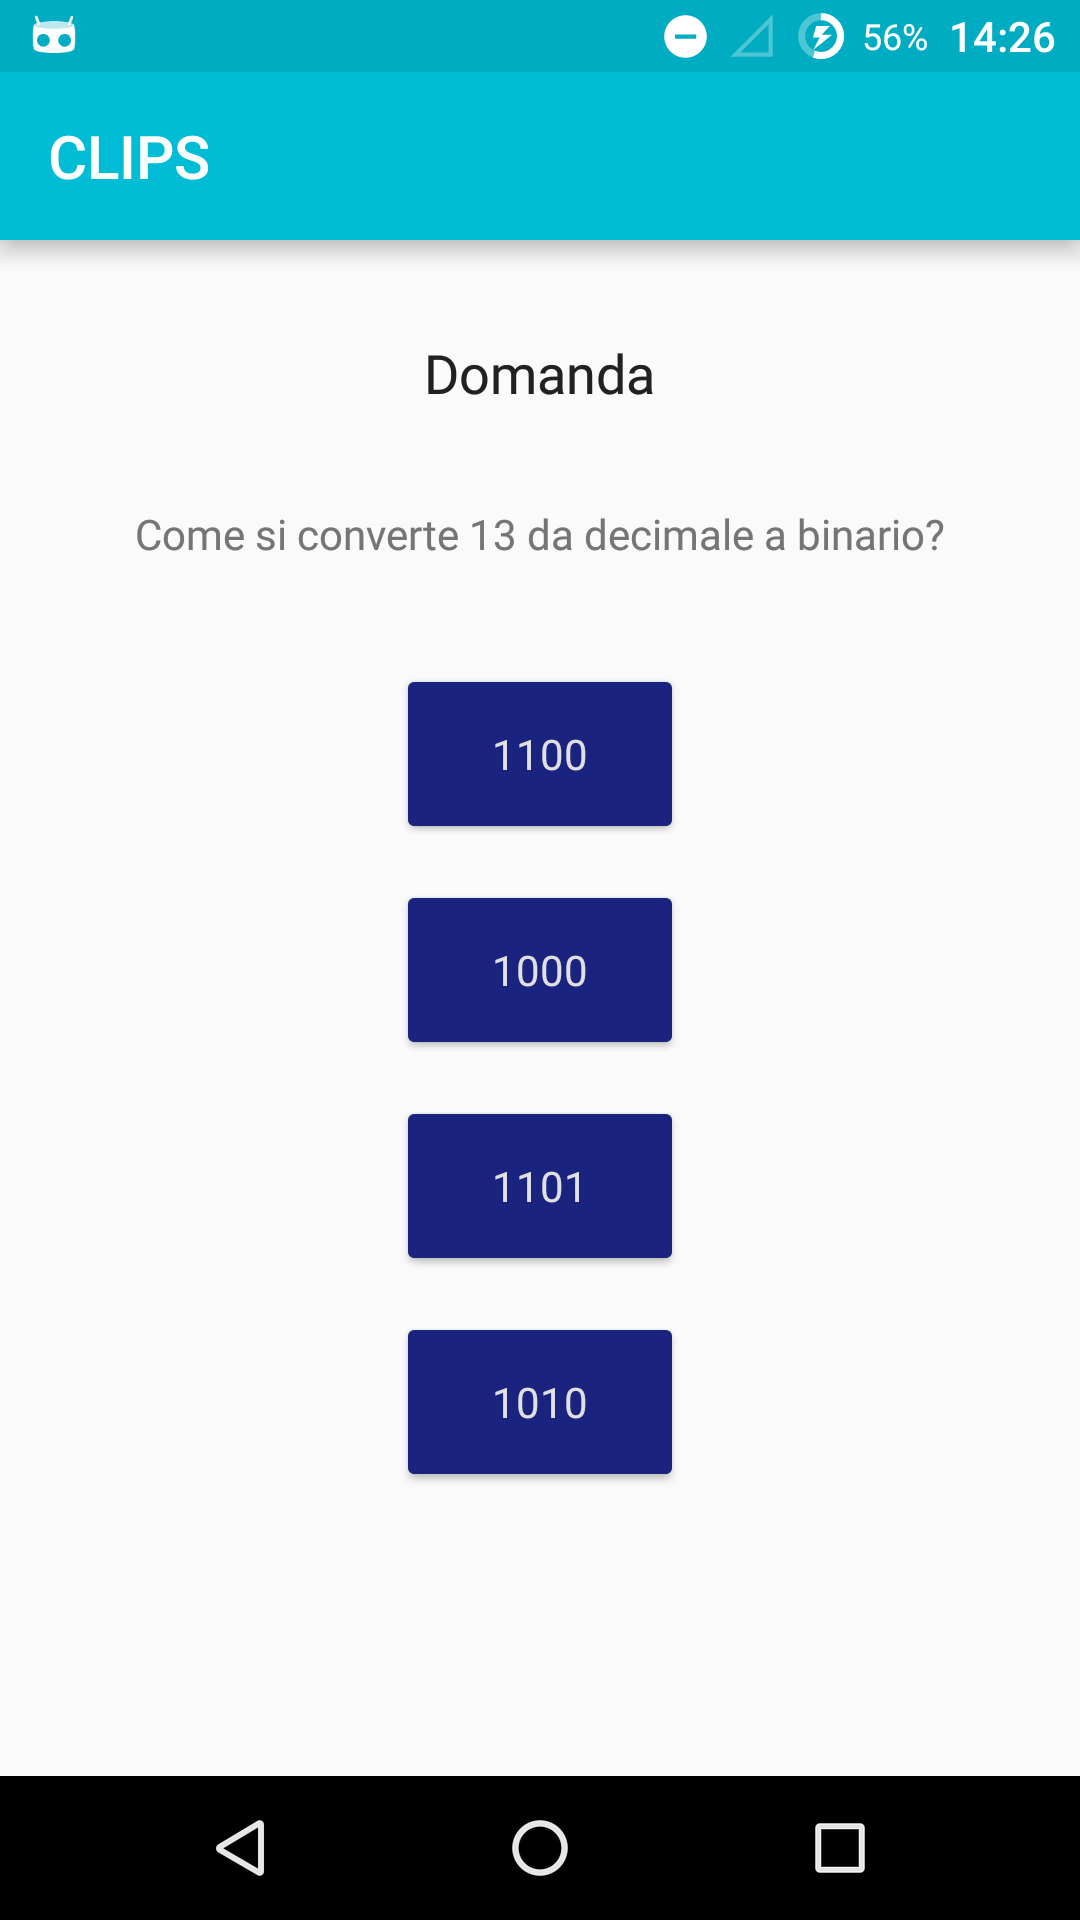
\includegraphics[scale=0.15]{screenshot/domanda}
	\caption{Schermata di visualizzazione domanda}
\end{figure}

Una volta che l'utente avrà risposto alla domanda verrà indirizzato ad una schermata in cui gli verrà detto se la risposta data è esatta o meno (figura 9). In caso affermativo gli verranno date indicazioni sulla prossima tappa da cercare.

\begin{figure}[!h]
	\centering
	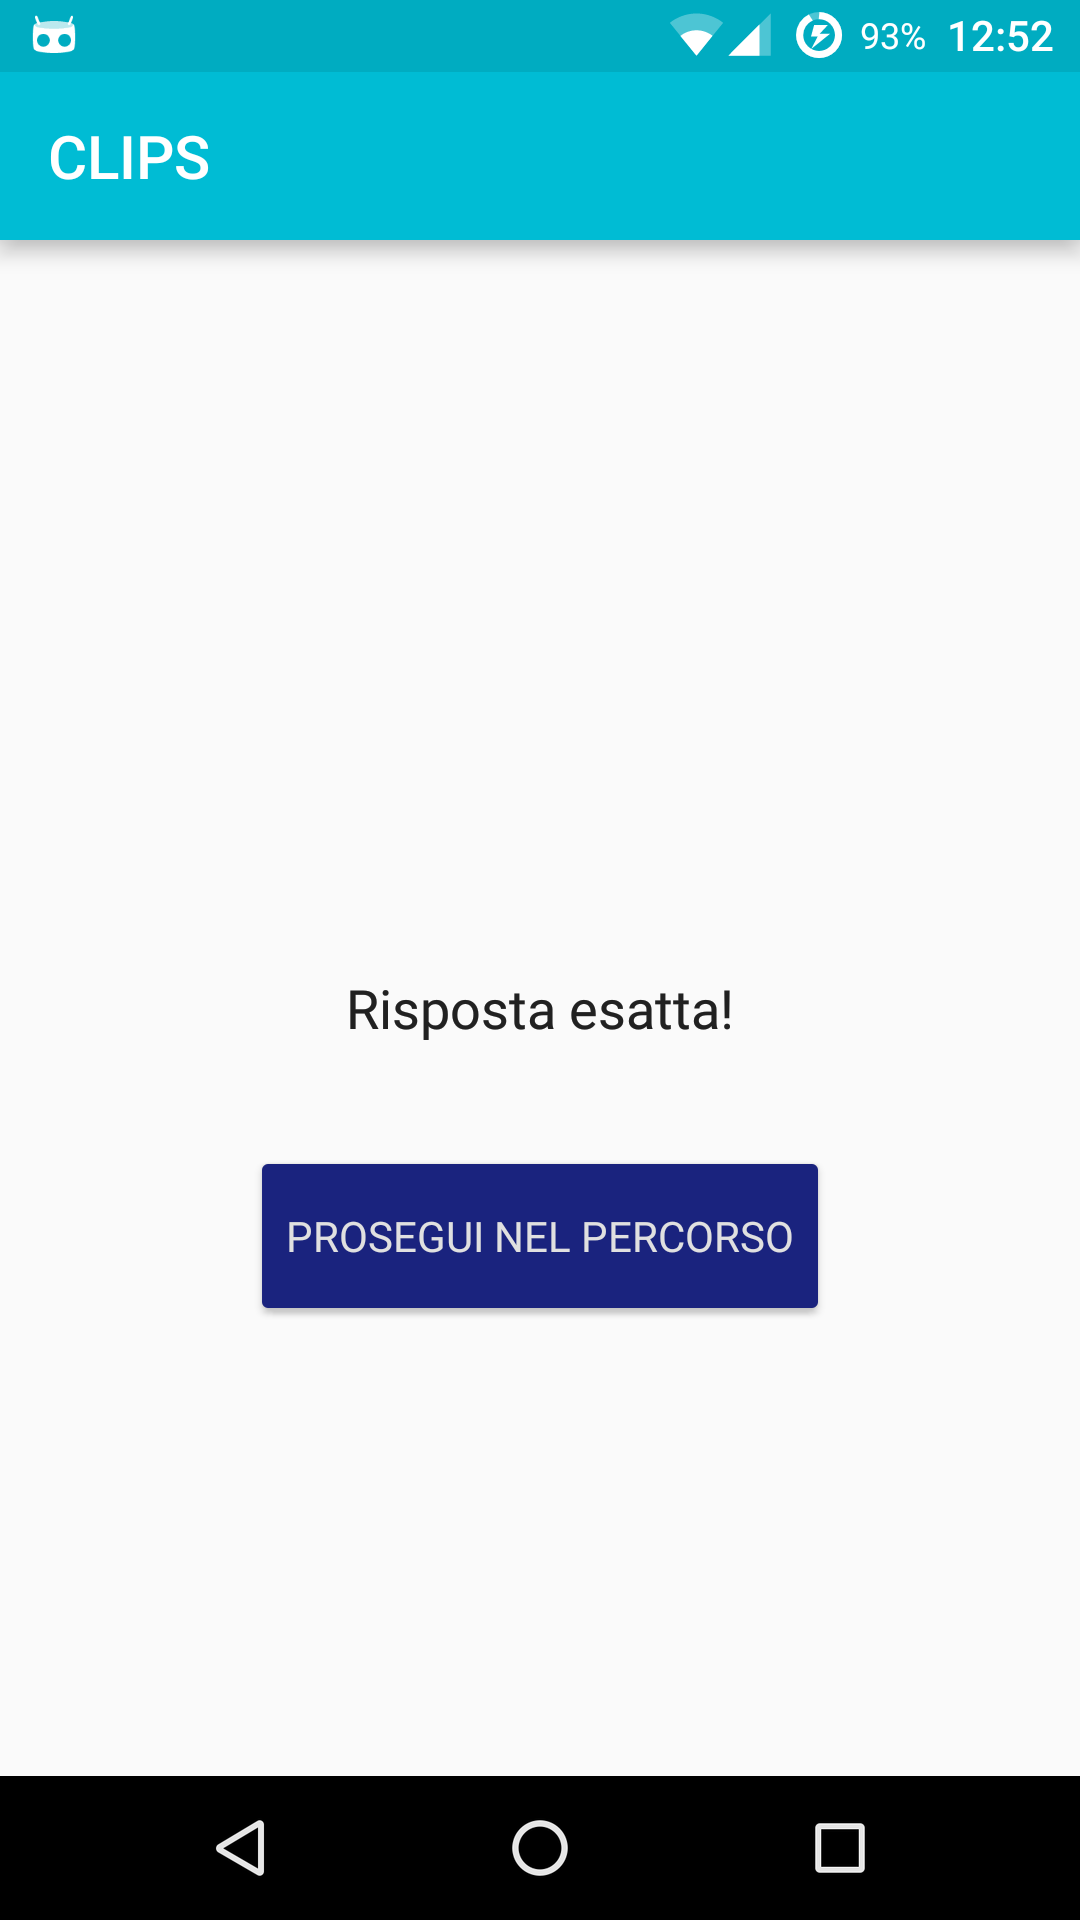
\includegraphics[scale=0.15]{screenshot/risultato_prova}
	\caption{Schermata di visualizzazione domanda}
\end{figure}